
\documentclass[%
 reprint,
%superscriptaddress,
%groupedaddress,
%unsortedaddress,
%runinaddress,
%frontmatterverbose, 
%preprint,
%preprintnumbers,
%nofootinbib,
%nobibnotes,
%bibnotes,
 amsmath,amssymb,
 aps,
%pra,
%prb,
%rmp,
%prstab,
%prstper,
%floatfix,
]{revtex4-2}

\usepackage{graphicx}% Include figure files
\usepackage{dcolumn}% Align table columns on decimal point
\usepackage{bm}% bold math
\usepackage{caption}
\usepackage{subcaption}
\usepackage{float}
\usepackage{placeins} 
\usepackage[pdftex,
            pdfauthor={Cano Jones, Alejandro},
            pdftitle={Numerical Correspondence Between Paths in Causal Sets and Geodesics at the Continuum through (1+1) FLRW backgrounds.},
            pdfsubject={Path-Geodesic Correspondence Causal Set Theory},
            pdfkeywords={Quantum Gravity, Numerical Methods}]{hyperref}
%\usepackage{hyperref}% add hypertext capabilities
%\usepackage[mathlines]{lineno}% Enable numbering of text and display math
%\linenumbers\relax % Commence numbering lines

%\usepackage[showframe,%Uncomment any one of the following lines to test 
%%scale=0.7, marginratio={1:1, 2:3}, ignoreall,% default settings
%%text={7in,10in},centering,
%%margin=1.5in,
%%total={6.5in,8.75in}, top=1.2in, left=0.9in, includefoot,
%%height=10in,a5paper,hmargin={3cm,0.8in},
%]{geometry}

\begin{document}


\title{Numerical Correspondence Between Paths in Causal Sets and Geodesics at the Continuum through (1+1) FLRW backgrounds.}% Force line breaks with \\
\thanks{Not peer-reviewed.}%

\author{Cano Jones, Alejandro}

 \email{alexcanojones@gmail.com}




\date{\today}% It is always \today, today,
             %  but any date may be explicitly specified

\begin{abstract}
\begin{description}
\item[Abstract]
This study aims to shed some light into the possibility of modelling spacetime manifolds as discrete sets of points with a causal structure (Causal Set Theory). In particular, how one might recover trajectories in a manifold from this discrete model. To do so, this work presents numerical evidence of a correspondence between the discrete and continuum trajectories under the standard cosmological background described by a FRLW metric manifold.
\end{description}
\end{abstract}

\maketitle

\section{Introduction}
The current mathematical description of spacetime passes through the mathematical notion of a Lorentzian manifold, under the assumption of a continuity of space and time. This model has grate advantages as well as observational and experimental evidence; allowing for a correct description of gravity and quantum field theories alike. The problem arises at the intent of quantizing general relativity (and thus, the spacetime manifold itself); whereas the usual canonical quantization approach generates ultraviolet divergences, problem known as the \textit{continuum catastrophe}.

Many other approaches have been proposed in an attempt to reconcile both gravity and quantum theories such as string theory, quantum loop theory or high derivatives gravity; the focus of this paper will be the proposal of describing spacetime itself as a discrete set of points alongside a causal relation: the theory of causal sets; which will be discussed more in depth bellow. For this model to be able to reproduce existing observational and experimental evidences; it would have to be a limiting case of general relativity, as such, trajectories on a Lorentzian manifold must be reproduced correctly in this setting. The truth of the last idea, is not completely known, and other studies have tried to present evidence for it, such as \cite{Original_Idea}; whose methodology has been reproduced in this work.
\subsection{Causal Sets: An Axiomatic Definition}
As previously stated, the theory of causal sets, will describe spacetime as a set of points (or causet) $\mathcal{C}$ alongside a partial ordered (causal) relation $(\mathcal{C}\,,\;\preceq)$. To completely describe the model, one must add the following set of axioms to be enforced to the two previous fundamental concepts. Said requested properties are (a) \textit{Reflexivity} $\forall x\in\mathcal{C}\,,\; x\preceq x$; (b) \textit{Transitivity} $\forall x,y,z\in\mathcal{C}\,,\;(x\preceq y\,\land\,y\preceq z)\implies x\preceq z$; (c) \textit{Acyclicity} $\forall x,y\in\mathcal{C}\,,\;(x\preceq y\,\land\,y\preceq x)\implies x=y$ and (d) \textit{Local Finiteness} $\forall x,y\in\mathcal{C}\,,\; |\{z\in\mathcal{C}\,|\, x\preceq z\preceq y\}|< \aleph_0$.


\subsection{Path and Geodesic Correspondence}
Alongside the notion of causal sets, two more definitions are needed. Considering two points $x,y\in\mathcal{C}$; the relation $x\preceq y$ is said to be a  \textit{link} if it is irreducible, meaning that $\not\!\exists z\!\in\mathcal{C}$ such that $x\preceq z\preceq y$. In addition, a \textit{Path}, is an ordered set $(x_0,\,x_1\,\cdots,\,x_n)\in\mathcal{C}^n$ in which  $x_i\preceq x_{i+1}$ is a link.

The connection between paths and geodesics along a metric manifold, was made by Myrheim \cite{Conjecture} in his length conjecture, stating that the length of the longest path between two related elements in a causet is the most natural analogue for the geodesic length (since the latter is also maximal in a continuum). The idea being, that one would recover the trajectory in the limit of an infinite point density over the manifold.  Although this conjecture has been proven correct \cite{FlatProof} in the case of Minkowskian backgrounds; the generalization over curved metric spaces has not been founds; this work therefore will look for evidence of the truthfulness of the conjecture for (1+1) FLRW metric spaces, described by a line element
\begin{equation}\label{eq: FLRW}
    \text{d}s^2=-c^2\text{d}t^2+a(t)\frac{\text{d}r^2}{1-\kappa r^2}\,,
\end{equation}
whereas $a(t)$ is a scale factor and $\kappa\in\{0,\pm 1\}$ the spacial curvature.
\section{Causets: Generation Methodology}
The general definition of a causet does not need to be directly related with a specific manifold; in fact, a given causet $\mathcal{C}$ can be well approximated by two (or more) distinct manifolds $\mathcal{M}$ and $\mathcal{M}'$, although they must be approximately isometric. Therefore a method to produce a causet from a manifold is needed; which its commonly known as a \textit{sprinkling}.
\subsection{Sprinkling}
A sprinkling can be described as the method in which the location of a point of $\mathcal{C}$ over a manifold $\mathcal{M}$ is chosen. A naive idea would be to place the points evenly spread throughout the manifold; the problem with this method is that its not invariant under Lorentzian transformations. The best  mapping between $\mathcal{C}$ and $\mathcal{M}$ seems to be obtained via a \textit{Poisson} process\cite{Bombelli}; in which a given region of volume $V$, $n$ points will be spread (following a flat random distribution) over this region; where the number of points on said volume follows a Poisson distribution of the form
\begin{equation}
    P_\rho(n,V)=\frac{(\rho V)^{n}}{n!}e^{-\rho V}\,,
\end{equation}
in which $\rho$ is described as the point number density; allowing to compute that the average number of points would be $\langle n\rangle=\rho V$. The best embedding is obtained by considering a disjoint foliation $\{\mathcal{M}_i\subset\mathcal{M}\,|\,\mathcal{M}_n\cap\mathcal{M}_m=\emptyset\,,n\not=m\}$ of the manifold $\mathcal{M}$; in which for each the poisson process is taken, with volumes
\begin{equation}
    V_{\mathcal{M}_i}=\int_{\mathcal{M}_i}\sqrt{-g}\,\text{d}^dx\,.
\end{equation}
Taking the metric tensor proposed in \ref{eq: FLRW}, results are given by
\begin{equation}
    V_{\mathcal{M}_i}=\frac{1}{\sqrt{\kappa}}\arcsin{\left(r\sqrt{\kappa}\right)}\Big|_{r_i}^{r_{i+1}}\int_{t_i}^{t_{i+1}}a(t)\text{d}t\,.
\end{equation}
With this, the set of points $\mathcal{C}$ is described, although the causal relation isn't specified.
\subsection{Causal Structure}
Since the causet in play is supposed to be a discretization of a particular manifold, it seems natural to assume that the two must have the same causal structure. For the former, it will be described by the partial order $\preceq$; whereas for the latter, causality is determined by null trajectories. It is said that two points in a Lorentzian manifold are causally connected if there exists a null geodesic connecting them; for the metric manifold in question (eq.\ref{eq: FLRW}), this trajectory can be obtained imposing $\text{d}s^2=0$, resulting in
\begin{equation}
    \left(\frac{\text{d}r}{\text{d}t}\right)^2=\frac{c^2}{a(t)}\sqrt{1-\kappa r^2}\,;
\end{equation}
although the causality of two points can be determined, its order has not been imposed. Another condition must be met: for two points $x,y\in\mathcal{C}$ to be ordered through $x\preceq y$, the temporal coordinate of $y$ must be grater than the corresponding for $x$; meaning that:
\begin{equation}
    x\preceq y \iff\exists \gamma(\tau):[0,1]\to\mathcal{C}\,s.t. \gamma(0)=x\,\land\,\gamma(1)=y\,,
\end{equation}
whereas $\gamma(\tau)$ its the trajectory over the manifold $\mathcal{M}$.

This definition allows to create a connection between light cones in the $\mathcal{M}$ and $\mathcal{C}$; in which we can describe the \textit{causal future} of a point $x\in\mathcal{C}$ as the set
\begin{equation}
    F(x)\equiv\left\{y\in\mathcal{C}\,|\,x\preceq y\right\}
\end{equation}

To have a notion of the geometric causal structure, a Hasse Diagram (FIG.\ref{fig: Hasse Siagram}) can be employed; all points $x\in\mathcal{C}$ are represented in their corresponding spacetime coordinates and are to be understood as nodes on a graph, for winch an edge will be drawn between two nodes $x,y\in\mathcal{C}$ if $x\preceq y$ is a link.
\begin{figure}[h]
\centering
\begin{subfigure}{.4\textwidth}
  \centering
  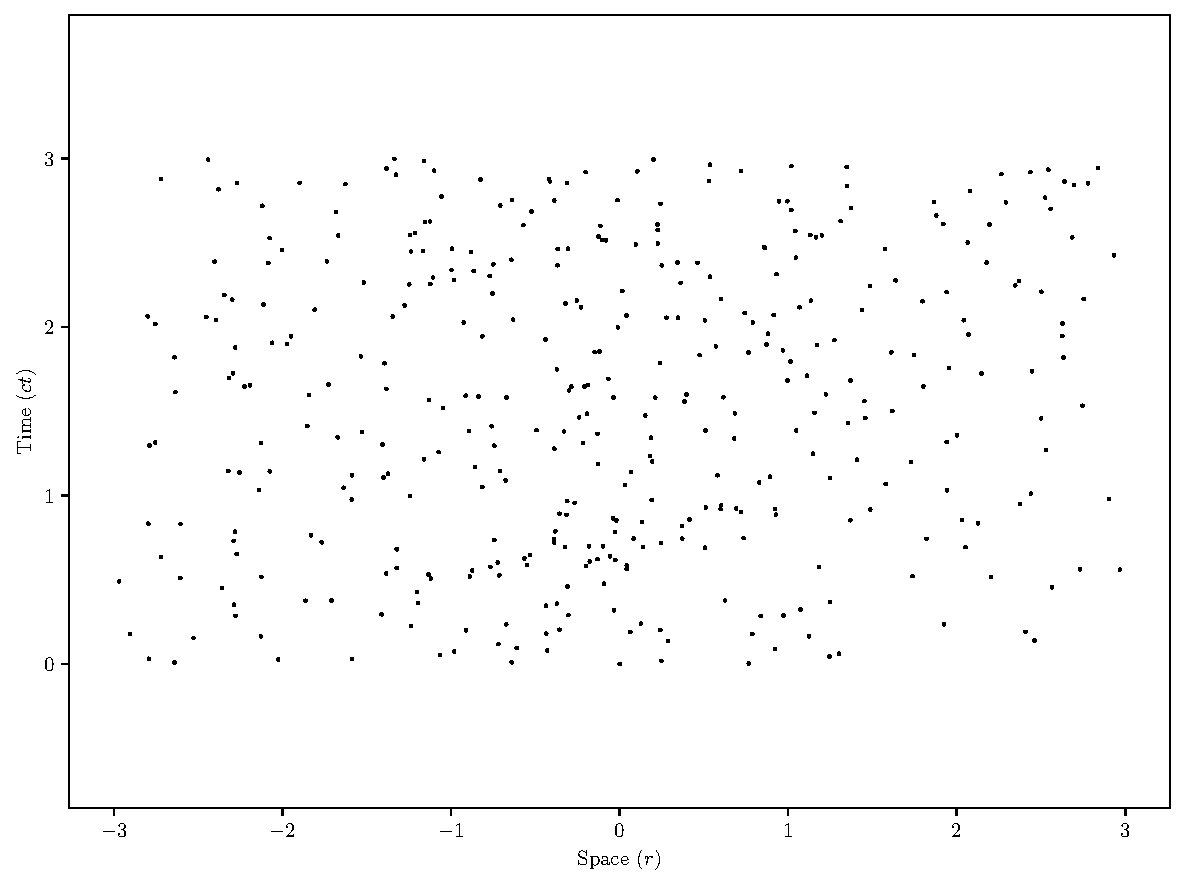
\includegraphics[width=\linewidth]{Images/Causet.pdf}
  \caption{Scatterplot of the causet.}
  \label{fig: causet scatter}
\end{subfigure}%
\begin{subfigure}{\textwidth}
    \centering
\end{subfigure}
\begin{subfigure}{.4\textwidth}
  \centering
  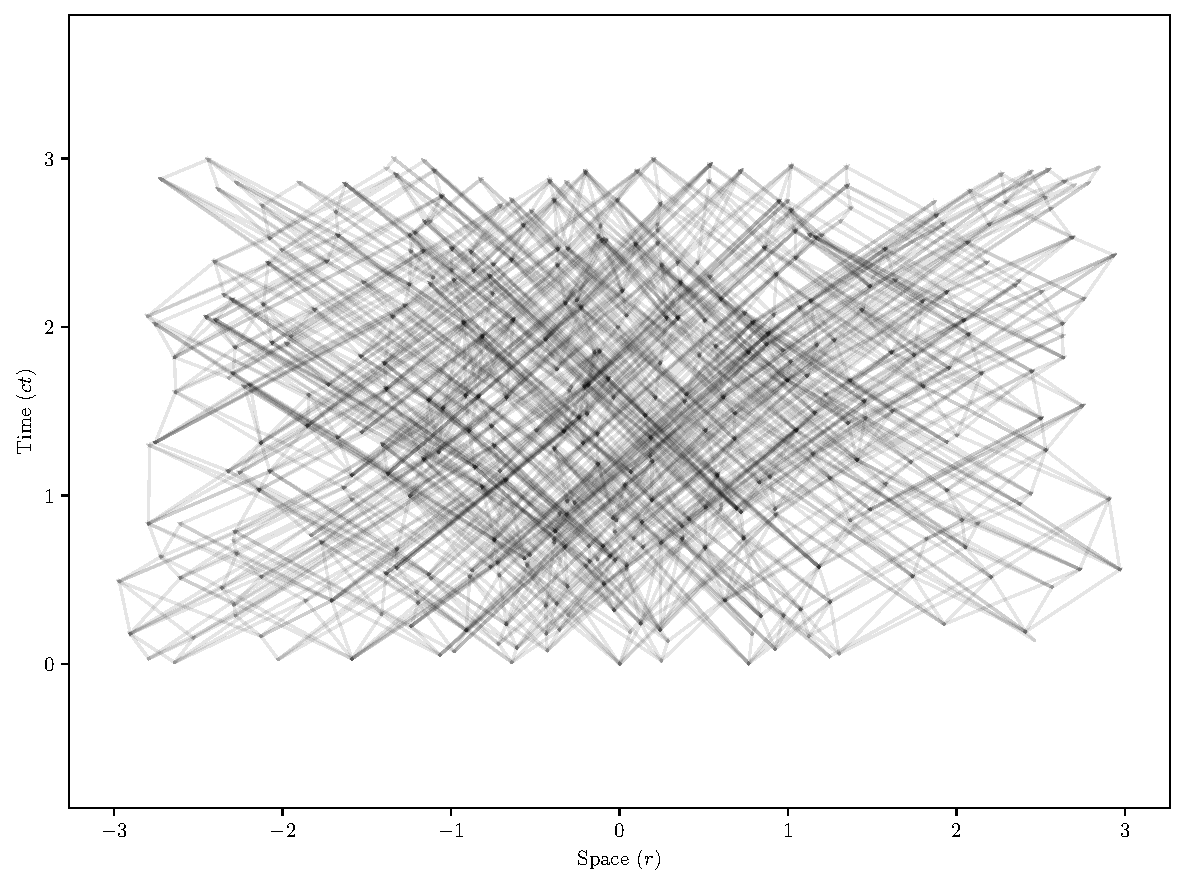
\includegraphics[width=\linewidth]{Images/Hasse_Diagram.pdf}
  \caption{Hasse Diagram on the same causet.}
  \label{fig: Hasse Siagram}
\end{subfigure}
\caption{Causet $(\mathcal{C},\preceq)$ over hyperbolic space with $\langle n\rangle=350$.}
\label{fig: Hyperbolic}
\end{figure}
\FloatBarrier

Once a causet $(\mathcal{C},\preceq)$ has been completely determined from a metric manifold $\mathcal{M}$, an analysis of theoretical propositions can be individually be check through numerical methods.

\section{Implementation and Results}
The algorithm implementation of the objective we face; must start by completely characterising the parameters to consider; which would include: the metric space given by equation \ref{eq: FLRW}, the submanifold region $\mathcal{M}$ to be considered (since an infinite manifold would be numerically not possible), a number point density $\rho$ (which is more easily implemented as the expected number of points in the causet) and finally the continuum geodesic to be compared to. The python code employed in this work can be found at the \cite{GitHub} GitHub repository.

Once the proper characterization of the simulation has been made, the first step is the creation of the causet $\mathcal{C}\subset\mathcal{M}$, which is done using the sprinkling method previously presented, alongside two points of the continuum geodesic; this would result in something similar to FIG. \ref{fig: causet scatter}. Causal structure $\preceq$ follows, by checking whether for two points $x,y$ in the causet $\mathcal{C}$, there is a null geodesic connecting them; if this is the case, then either $x\preceq y$ or $y\preceq x$ (depending on the temporal ordering). This causal structure is coded into a graph $\mathcal{G}$ represented by a Hasse Diagram as in FIG. \ref{fig: Hasse Siagram}.

The previous steps would have prepared the dataset for analysis; which is to compare paths and geodesics. Since there are at least two points in common between the causet and the geodesic, those will be considered the starting and ending points of the path (again, depending on the temporal ordering). Here, all paths between the starting anmd ending points are computed and compared, in order to find the maximal lenth paths (which might not be unique). All paths and geodesic are compared as in FIG. \ref{fig:Spherical}.
\begin{figure}
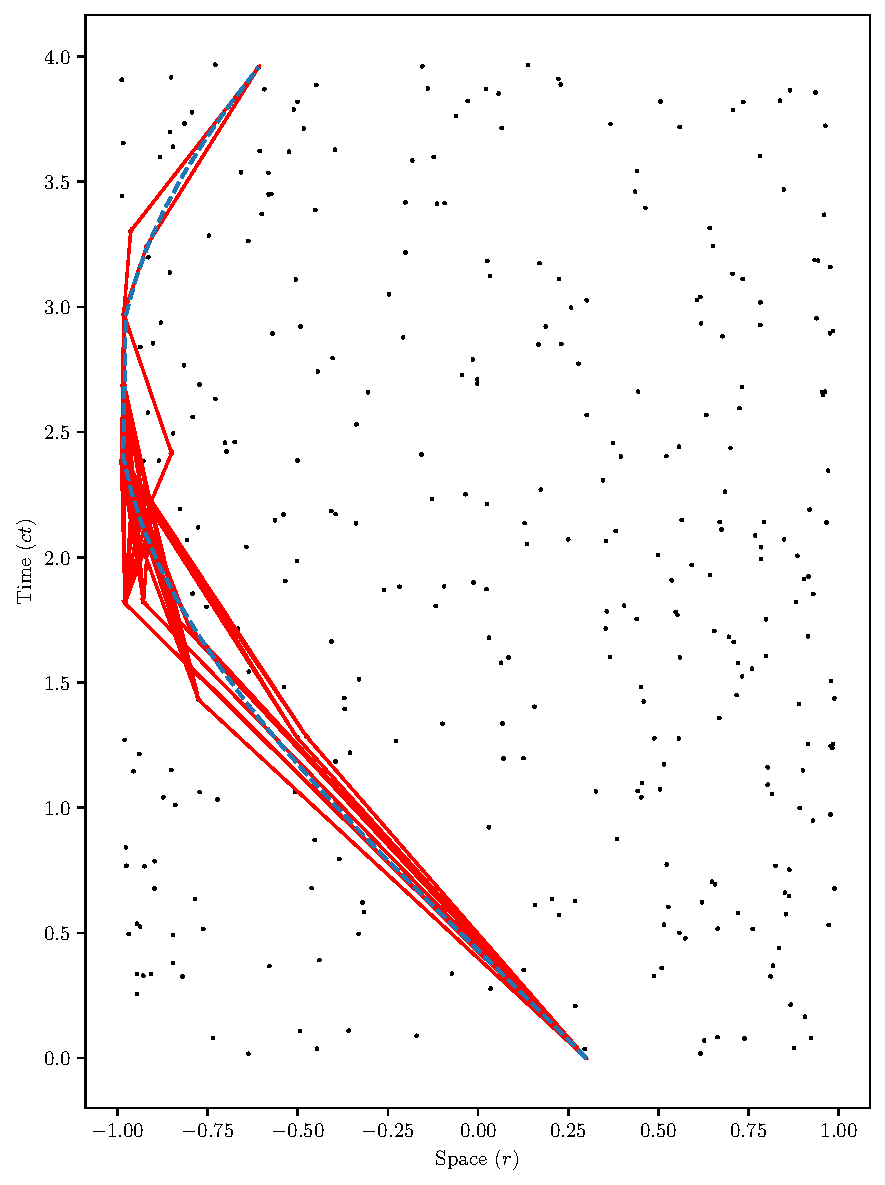
\includegraphics[width=\linewidth]{Images/Correspondence.pdf}% Here is how to import EPS art
\caption{\label{fig:Spherical} Numerical correspondence between discrete paths (red) and continuum geodesic (blue) over an spherical background with $\langle n\rangle=350$.}
\end{figure}
\FloatBarrier
\section{Conclusions}
Through a number of attempts, all maximal paths in a causet do seem to approximate the continuum geodesics. Although we have a good visual fit, future works should also implement a $\chi^2$ test in order to properly compare the two of them. Moreover, the path-geodesic correspondence should be studied in the continuum limit, recovered by the limit $\rho\to \infty$. Therefore this algorithm and implementation should be the grounds for a larger data analysis of the dependence of $\langle\chi^2\rangle$ with $\rho$; expecting to be a decreasing function, just as in the works by \cite{Original_Idea}.
\vfill
\nocite{*}
\bibliography{apssamp}

\end{document}
